\section{Module 8. Skull stripping}
\section{Module 8. Skull stripping}
Module 8 has implemented own class \textbf{SkullStripping} with consist of methods required to skull strip the image.
Implemented methods:
\begin{itemize}
    \item {\textbf{def recon (self,marker,mask)} - which is used to grey image reconstruction based on morphological grey dilation, \textbf{input:} marker - image to reconstruction, mask - mask image \textbf{output:} recon - reconstructed image}
    \item {\textbf{def strel (self, type, size)} - which creates an logical array to morphological operation,\textbf{input:} type - string with type structuring element, two option implemented 'disk' and 'array', size - array size \textbf{output:} array - a logical array}
    \item {\textbf{def csf counting(self)} - which estimates CSF based on histogram \textbf{input:} self - class SkullStripping object consisting of MRI image  \textbf{output:}  csf - estimated CSF parameter}
    \item {\textbf{def binarization(self, image, threshold, upper=1, lower=0)} - which changes grey image to binary image
    \textbf{input:} image - image to binarization, threshold - threshold for binarization, upper - value of pixels over the threshold, lower - value of pixels under the threshold, output: bin image - binary input image}
    \item {\textbf{def radius counting(self, bin image} - which estimates BR and ratio diameter in axis x to diameters in axis y \textbf{input:} bin image - binary image \textbf{output:} r - BR estimated parameter, st - ratio}
    \item {\textbf{def preprocessing(self)} - which consist methods to estimate CSF, BR, ratio, and COG and cropp image based on BR parameter \textbf{input:} self - class SkullStripping object consisting of MRI image \textbf{output:} cropped image - image cropped based on BR parameters, csf - estimated CSF parameter, COG - coordinates of the centroid of the brain, r - estimated BR parameter, st - ratio diameters in axis x to diameters in axis y
    \item {\textbf{def grad mag sobel(self, image)} - which computes gradient magintude using the Sobel edge mask\textbf{input:} image - input image \textbf{output:}  gradmag - gradient magintude input image}
    \item {\textbf{def anisodiff(self, image, niter=1,kappa=50,gamma=0.1, step(1.,1.),option=1)} - which filter using of anisotropic diffusion filter \textbf{input:} image - input image, niter- amount of iteration, kappa, gamma, step - parameters of filter, option - method of filtering  \textbf{output:} image out - image after filtration}
    \item {\textbf{def edges marr hildreth(self, image, sigma)} - which is the Marr-Hidreth edge detector \textbf{input:} image - input image, sigma - edge detector parameter \textbf{output:} zero crossing - binary image with black boundaries of object in image and white the others object}
    \item {\textbf{def background marker(self, preproc image, csf)} - which marks the background objects \textbf{input:}preproc image - image especially after preprocessing, csf - CSF parameter \textbf{output:} bgm - markers of background}
    \item {\textbf{def foreground marker(self, preproc image, csf)} - which marks the foreground objects \textbf{input:} preproc image - image especially after preprocessing, csf - CSF parameter \textbf{output:} fgm4 - markers of foreground}
    \item {\textbf{def watershed(self, preproc image, csf, cog)} - which is used to marker-controlled watershed segmentation \textbf{input:}preproc image - image especially after preprocessing, csf - CSF parameter, cog - COG parameter \textbf{output:} brain - skull stripping mask}
    \item {\textbf{def bse(self, cog} - which is used to brain surface extraction \textbf{input:} self - class SkullStripping object consisting of MRI image, cog - COG parameter \textbf{output:} brain - skull stripping mask}
    \item {\textbf{def run(self, verbose=False)} - which is used to run module08 \textbf{input:}self - class SkullStripping object consisting of MRI image, verbose - True or False plotting result of method  \textbf{output:} skull stripping mask - output of the module}
\end{itemize}
To connect with project it is implemented function:
\begin{itemize}
    \item {\textbf{def main8(mri input,verbose=Flase)}}
\end{itemize}
Method \textbf{run()} scheme:
\begin{enumerate}
    \item {Preprocessing compute CSF, COG, BR, ratio, and cropped image using of \textbf{preprocessing()}.}
    \item {Checking BR and ratio to eliminate slice without the brain tissue.}
    \item {Brain Surface Extraction using of \textbf{bse()}.}
    \item {Checking skull stripping mask to eliminate too large mask based on BR parameters. If it is not too large return skull stripping mask.}
    \item {\textbf{(OPTIONAL if mask from BSE is too large.)} Marker-controlled watershed segmentation using of \textbf{watershed()}.}
\end{enumerate}

Evaluation of Module 8's results are presented on figures bellow:
\begin{figure}[H]
\centering{}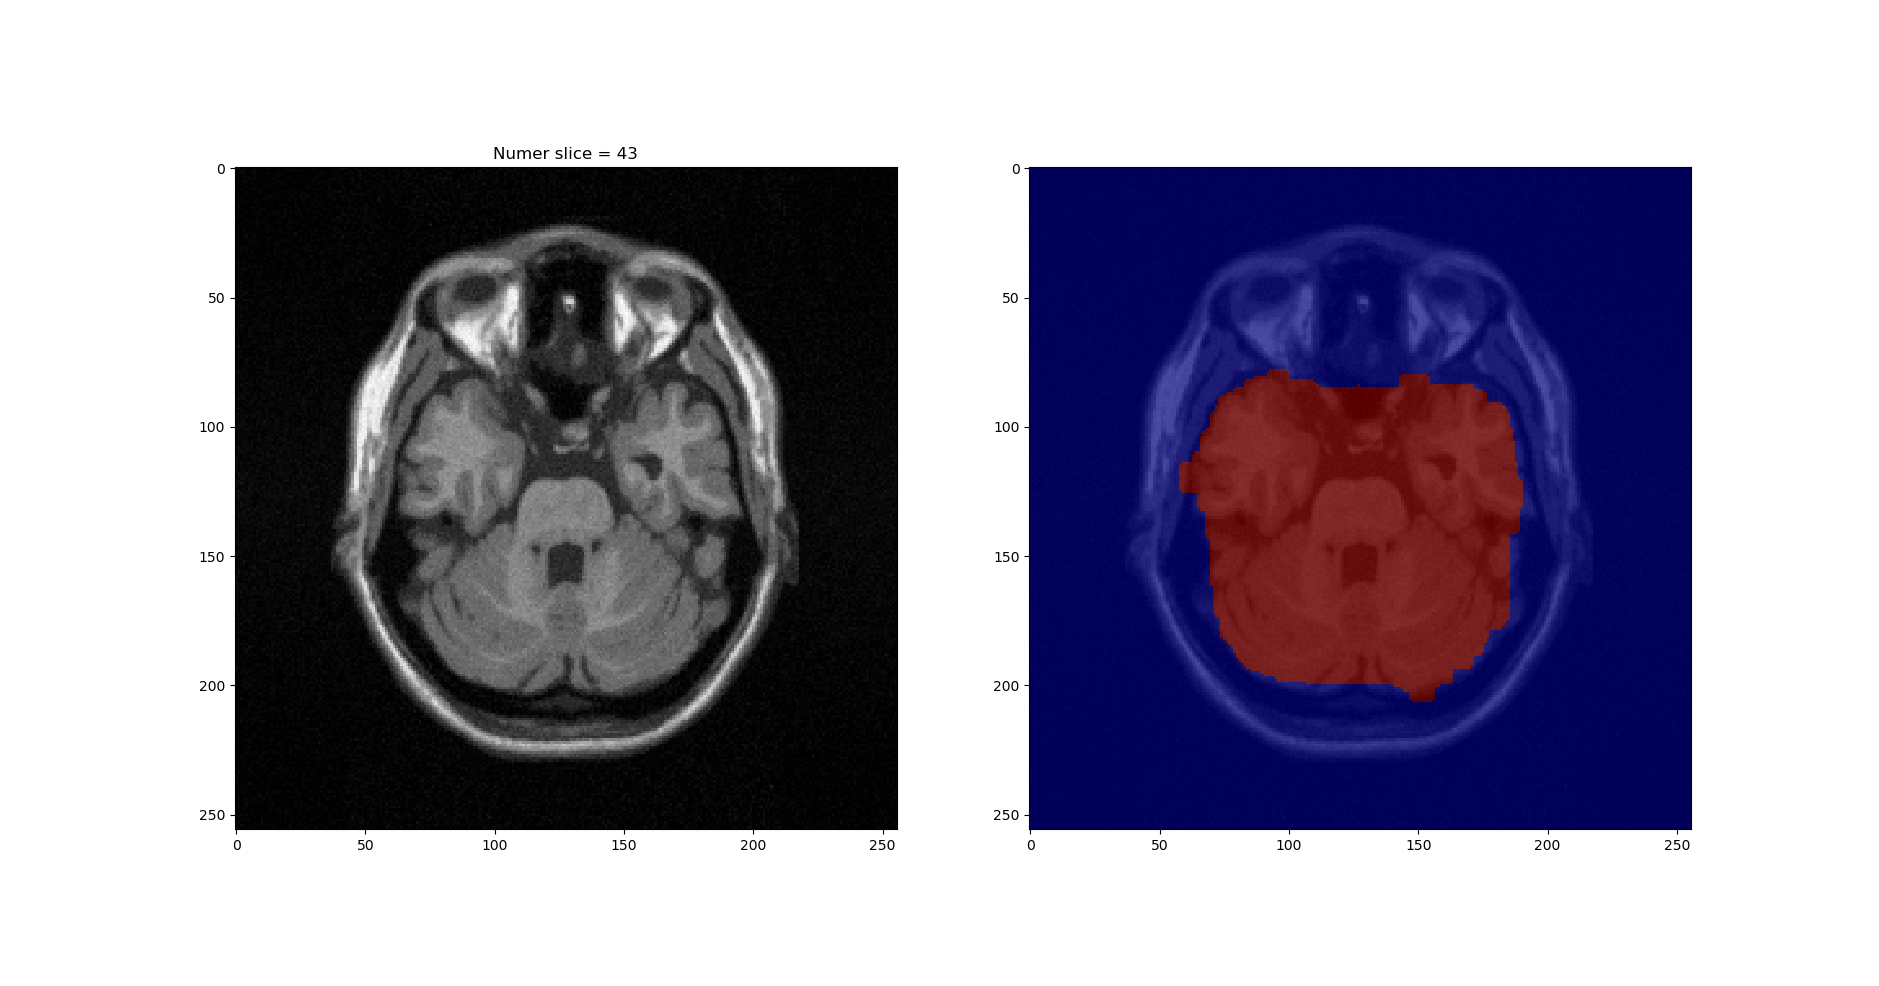
\includegraphics[scale=0.3]{figures/M8_Figure_1.png}\caption{MRI image with eyes and input image with skull stripping mask}.
\label{fig:figures/Module8_Figure_1}
\end{figure}
\begin{figure}[H]
\centering{}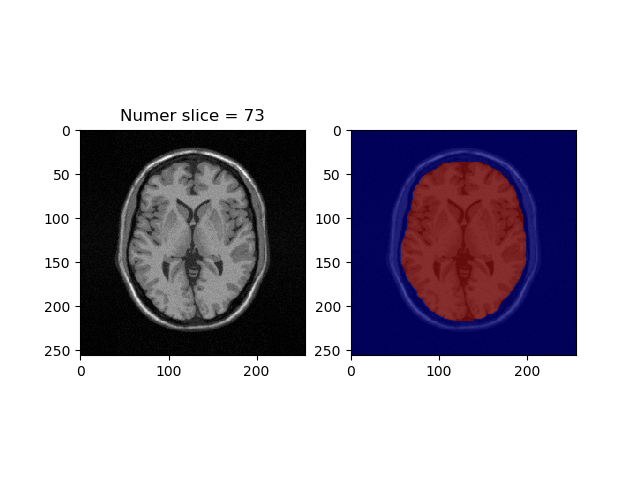
\includegraphics[scale=0.8]{figures/M8_Figure_1-3.png}\caption{MRI image and input image with skull stripping mask}.
\label{fig:figures/Module8_Figure_2}
\end{figure}
\begin{figure}[H]
\centering{}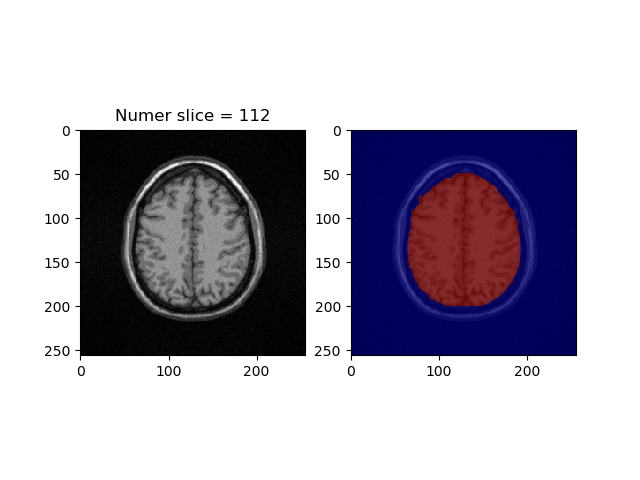
\includegraphics[scale=0.8]{figures/M8_Figure_1-4.png}\caption{MRI image and input image with skull stripping mask}.
\label{fig:figures/Module8_Figure_3}
\end{figure}
\begin{figure}[H]
\centering{}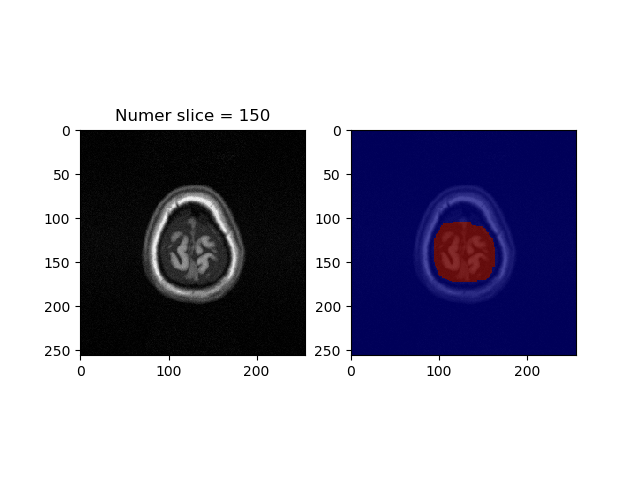
\includegraphics[scale=0.8]{figures/M8_Figure_1-6.png}\caption{Image of upside part of brain and input image with skull stripping mask}.
\label{fig:figures/Module8_Figure_4}
\end{figure}